\documentclass{article}
\usepackage{listings}
\usepackage{xcolor}
\usepackage{enumitem}
\usepackage{graphicx}
\usepackage{amssymb}
\usepackage{bytefield}
\usepackage{forest}
\usepackage{tikz}
\usetikzlibrary{arrows.meta, positioning,trees}
\usepackage{float}
\usepackage{fancyhdr} % Custom headers/footers
\usepackage{colortbl}
\usepackage[left=0.6in, right=0.6in, top=1in, bottom=0.9in]{geometry}
\usepackage{indentfirst}
\usepackage{changepage, titlesec}
\usepackage{booktabs}
\usepackage{array}
\usepackage{adjustbox} % for adjustwidth
\usepackage{multicol} % for side-by-side columns
\setlength{\parindent}{1.5em} % Set indentation size (optional)
\usepackage{amsmath} % Required for align environment
\usepackage{xepersian}
\settextfont{Vazirmatn FD}
\setlatintextfont{Times New Roman} 


\pagestyle{fancy}     % Enable fancy headers
\fancyhf{}            % Clear default header/footer
\renewcommand{\headrulewidth}{0pt} % Disable default header line

\fancyhead[L]{\rule{\textwidth}{1pt}} % Manually add one line
\fancyfoot[C]{\thepage} % Page number in the center of the footer

\newcommand{\colorbitbox}[3]{%
	\rlap{\bitbox{#2}{\color{#1}\rule{\width}{\height}}}%
	\bitbox{#2}{#3}}
\definecolor{lightcyan}{rgb}{0.84,1,1}
\definecolor{lightgreen}{rgb}{0.64,1,0.71}
\definecolor{lightred}{rgb}{1,0.7,0.71}

\definecolor{codegreen}{rgb}{0,0.6,0}
\definecolor{codegray}{rgb}{0.5,0.5,0.5}
\definecolor{codepurple}{rgb}{0.58,0,0.82}
\definecolor{backcolour}{rgb}{0.95,0.95,0.92}

\lstdefinestyle{mystyle}{
	backgroundcolor=\color{backcolour},   
	commentstyle=\color{codegreen},
	keywordstyle=\color{magenta},
	numberstyle=\tiny\color{codegray},
	stringstyle=\color{codepurple},
	basicstyle=\ttfamily\footnotesize,
	breakatwhitespace=false,         
	breaklines=true,                 
	captionpos=b,                    
	keepspaces=true,                 
	numbers=left,                    
	numbersep=5pt,                  
	showspaces=false,                
	showstringspaces=false,
	showtabs=false,                  
	tabsize=2
}

\lstset{style=mystyle}

\ExplSyntaxOn
\NewDocumentCommand{\ReverseWords}{m}
{
	\seq_set_split:Nnn \l_tmpa_seq { ~ } { #1 } % Split words by spaces
	\seq_reverse:N \l_tmpa_seq % Reverse the order of words
	\seq_use:Nn \l_tmpa_seq { ~ } % Join words with spaces and output
}
\ExplSyntaxOff


\begin{document}
	\author{ مجتبی ملائی \\ ۴۰۱۳۱۳۸۳ }
	\title{ \huge { تکلیف چهارم}}
	\date{}
	\maketitle
\section{}	
\subsection{درخت تجزیه عبارت "MMLK"}
\begin{latin}
	

\begin{forest}
	for tree={
		draw,
		rounded corners,
		node options={align=center},
		grow'=south,
		child anchor=north,
		parent anchor=south,
		l=1.5cm,
		s sep=7mm,
		edge={->}
	}
	[S
	[D
	["M"]
	[D1
	["M"]
	[D1
	[$\varepsilon$]
	]
	]
	]
	[H
	["L"]
	[H1
	[$\varepsilon$]
	]
	]
	[T
	[$\varepsilon$]
	]
	[U
	["K"]
	]
	]
\end{forest}
\end{latin}
\vspace{1cm}

\subsection{مقدار ارتبیوت ها}
\begin{latin}
	

\begin{tabular}{@{}llc@{}}
	\toprule
	\textbf{Non-terminal} & \textbf{Production Used} & \textbf{Attribute Value} \\
	\midrule
	$S$   & $S \to D \; H \; T \; U$                   & $5 + 40 + (-5) + 5 = 45$ \\
	$D$   & $D \to \texttt{M} \; D1$                   & $5 + 0 = 5$ \\
	$D1$  & $D1 \to \texttt{M} \; D1$                  & $5 + (-5) = 0$ \\
	$D1$  & $D1 \to \varepsilon$                       & $-5$ \\
	$H$   & $H \to \texttt{L} \; H1$                   & $50 + (-10) = 40$ \\
	$H1$  & $H1 \to \varepsilon$                       & $-10$ \\
	$T$   & $T \to \varepsilon$                        & $-5$ \\
	$U$   & $U \to \texttt{K}$                         & $5$ \\
	\bottomrule
\end{tabular}
\end{latin}


\section{}



\subsection{الف) گراف  DAG}
\[
(((a + a) + (a + a)) + ((a + a) + (a + a)))
\]
\begin{latin}
	

\begin{center}
	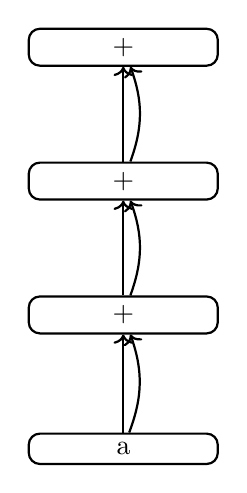
\begin{tikzpicture}[node distance=1.7cm, every node/.style={draw, rounded corners, minimum width=2.4cm, align=center}, ->, thick]
		
		\node (a) {a};
		\node (t1) [above of= a] {+};
		\node (t2) [above of= t1] {+};
		\node (t3) [above of= t2] {+};
		
		% Edges
		\draw (a) -- (t1);
		\draw (t1) -- (t2);
		\draw (t1) to[bend right=20] (t2);
		\draw (t2) -- (t3);
		\draw (t2) to[bend right=20] (t3);
		\draw (a) to[bend right=20] (t1);
		
	\end{tikzpicture}
\end{center}
\end{latin}
\vspace{1cm}

\subsection{ب) \lr{3AC}}
\begin{latin}
	

\begin{lstlisting}[language=, frame=single, basicstyle=\ttfamily]
	t1 = a + a
	t2 = t1 + t1
	t3 = t2 + t2
\end{lstlisting}
\end{latin}

\section{}
\begin{latin}
\subsection{Three-Address Code (3AC):  \( a + b \times c / e \, \hat{} \, f + b \times a \)}

\begin{lstlisting}[language=, frame=single, basicstyle=\ttfamily]
	t1 = e ^ f
	t2 = c / t1
	t3 = b * t2
	t4 = a + t3
	t5 = b * a
	t6 = t4 + t5

\end{lstlisting}



	

\subsection{ Quadruples for \( (a + b) \times (c + d) - (a + b + c) \)}

\begin{center}
	\begin{tabular}{@{}lllll@{}}
		\toprule
		\textbf{Index} & \textbf{Op} & \textbf{Arg1} & \textbf{Arg2} & \textbf{Result} \\
		\midrule
		(1) & + & a & b & t1 \\
		(2) & + & c & d & t2 \\
		(3) & * & t1 & t2 & t3 \\
		(4) & + & t1 & c & t4 \\
		(5) & - & t3 & t4 & t5 \\
		\bottomrule
	\end{tabular}
\end{center}


\subsection{3. Indirect Triple for \( a = -b \times (c / d) \)}

\begin{center}
	\begin{tabular}{@{}cccc@{}}
		\toprule
		\textbf{Index} & \textbf{Op} & \textbf{Arg1} & \textbf{Arg2} \\
		\midrule
		(0) & / & c & d \\
		(1) & minus & b &   \\
		(2) & * & (1) & (0) \\
		(3) & = & a & (2) \\
		\bottomrule
	\end{tabular}
	
	\vspace{0.5cm}
	
	\textbf{Pointer Table:}
	\vspace{0.2cm}
	
	\begin{tabular}{@{}ll@{}}
		P[0] & → (0) \\
		P[1] & → (1) \\
		P[2] & → (2) \\
		P[3] & → (3) \\
	\end{tabular}
\end{center}

\end{latin}


\section{}
\begin{latin}
\begin{lstlisting}[language=, frame=single, basicstyle=\ttfamily]
t1 = B1 and B2
t2 = not t1
t3 = B1 or B2
t4 = t2 and t3
B.val = t4

\end{lstlisting}
\end{latin}

\section{}
\subsection{الف)}
\begin{latin}
	\begin{lstlisting}[language=, frame=single, basicstyle=\ttfamily]
L1:   ifFalse x > 0 goto L5       ; check first part of &&  
ifFalse x < 100 goto L5     ; check second part of &&  
t1 = x + 1                  
x = t1                      
ifFalse x > 20 goto L3      
t2 = x + 2                  
x = t2                      
goto L4                     
L3:   t3 = x + 3                  
x = t3                      
L4:   goto L1                     
L5:
\end{lstlisting}
\end{latin}

\subsection{ب)}
\begin{latin}



\begin{align*}
	\text{begin} &= \text{newlabel()} \quad                      &\text{(Start of the loop body)} \\
	S_1.\text{next} &= \text{begin} \quad                        &\text{(Back edge to condition check)} \\
	B.\text{true} &= \text{begin} \quad                          &\text{(Loop again if condition is true)} \\
	B.\text{false} &= S.\text{next} \quad                        &\text{(Exit loop if condition is false)} \\
	S.\text{code} &= \text{label(begin)} \ || \ S_1.\text{code} \ || \ B.\text{code} \ ||\text{gen('goto begin')} \\
\end{align*}

\end{latin}


\section{}




\begin{latin}
	

\subsection{3AC}
\begin{align*}
	(1) &\quad t := 0 \\
	(2) &\quad i := 0 \\
	(3) &\quad L1: \quad \text{if } i > 10 \ \text{goto} \ L4 \\
	(4) &\quad t := t + i \\
	(5) &\quad i := i + 1 \\
	(6) &\quad \text{goto } L1 \\
	(7) &\quad L4: \quad x := t
\end{align*}
\subsection{}

\begin{align*}
	B_1 &: (1)\ t := 0 \quad (2)\ i := 0 \\
	B_2 &: (3)\ \text{if } i > 10 \ \text{goto} \ L4 \\
	B_3 &: (4)\ t := t + i \quad (5)\ i := i + 1 \quad (6)\ \text{goto } L1 \\
	B_4 &: (7)\ x := t
\end{align*}
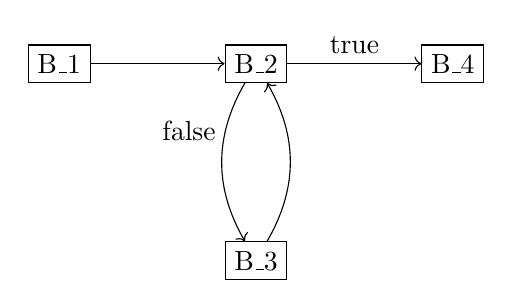
\begin{tikzpicture}[->, node distance=2.5cm, auto]
	\node[draw, rectangle] (B1) {B\_1};
	\node[draw, rectangle, right of=B1] (B2) {B\_2};
	\node[draw, rectangle, below of=B2] (B3) {B\_3};
	\node[draw, rectangle, right of=B2] (B4) {B\_4};
	
	\path (B1) edge (B2);
	\path (B2) edge[bend right] node[left, pos=0.3] {false} (B3);
	\path (B2) edge node {true} (B4);
	\path (B3) edge[bend right] (B2);
\end{tikzpicture}

\end{latin}

\section{}


\subsection{الف) }

\begin{latin}
	\begin{enumerate}
		\item READ(A)
		\item READ(B)
		\item C = A + B
		\item A = A + B          \quad // حذف شد (مشترک با 3)
		\item B = C * D
		\item T1 = C * D         \quad // حذف شد (مشترک با 5)
		\item T2 = T1 + C
		\item F = A + B          \quad // حذف شد (مشترک با 3)
		\item C = F + B
		\item G = A + B          \quad // حذف شد (مشترک با 3)
		\item T3 = F + B
		\item T4 = C * D         \quad // حذف شد (مشترک با 5)
		\item T5 = T3 + T4
		\item WRITE(T5)
	\end{enumerate}
\end{latin}

بنابراین کد جدید و بهینه‌شده به صورت زیر خواهد بود:

\begin{latin}
	\begin{enumerate}
		\item READ(A)
		\item READ(B)
		\item C = A + B
		\item B = C * D
		\item T2 = B + C
		\item C = C + B
		\item T3 = C + B
		\item T5 = T3 + B
		\item WRITE(T5)
	\end{enumerate}
\end{latin}

\subsection{ب) }

در کد اولیه، خطوطی که مقدارشان استفاده نشده‌اند و فقط مقداردهی کرده‌اند (و اثر در خروجی ندارند)، عبارت‌اند از:

\begin{latin}
	4, 6, 8, 10, 12
\end{latin}

\subsection{ج)}

\subsection*{الف) حذف عبارات مشترک (Common Subexpression Elimination)}

\begin{latin}
	\begin{enumerate}
		\item READ(A)
		\item READ(B)
		\item C = A + B
		\item A = A + B          \quad // حذف شد (مشترک با 3)
		\item B = C * D
		\item T1 = C * D         \quad // حذف شد (مشترک با 5)
		\item T2 = T1 + C
		\item F = A + B          \quad // حذف شد (مشترک با 3)
		\item C = F + B
		\item G = A + B          \quad // حذف شد (مشترک با 3)
		\item T3 = F + B
		\item T4 = C * D         \quad // حذف شد (مشترک با 5)
		\item T5 = T3 + T4
		\item WRITE(T5)
	\end{enumerate}
\end{latin}

بنابراین کد جدید و بهینه‌شده به صورت زیر خواهد بود:

\begin{latin}
	\begin{enumerate}
		\item READ(A)
		\item READ(B)
		\item C = A + B
		\item B = C * D
		\item T2 = B + C
		\item C = C + B
		\item T3 = C + B
		\item T5 = T3 + B
		\item WRITE(T5)
	\end{enumerate}
\end{latin}

\subsection*{ب) کدام جملات در کد اولیه توسط \lr{dead code elimination} حذف خواهند شد؟}

در کد اولیه، خطوطی که مقدارشان استفاده نشده‌اند و فقط مقداردهی کرده‌اند (و اثر در خروجی ندارند)، عبارت‌اند از:

\begin{latin}
	4, 6, 8, 10, 12
\end{latin}

\subsection{ج)}
در کد جدیدی که بعد از حذف عبارات مشترک تولید شد، تمام دستوراتی که باقی مانده‌اند، در ادامه مورد استفاده قرار گرفته‌اند و اثری در خروجی دارند. بنابراین:


	هیچ‌کدام از دستورات باقی‌مانده توسط DCE حذف نخواهند شد.



\section{}



\begin{tikzpicture}[
	every node/.style={draw, circle, font=\scriptsize, minimum size=5mm, inner sep=1pt},
	edge from parent/.style={draw, -latex},
	sibling distance=10mm,
	level distance=12mm,
	level 1/.style={sibling distance=60mm},
	level 2/.style={sibling distance=20mm},
	level 3/.style={sibling distance=15mm},
	level 4/.style={sibling distance=8mm},
	]
	
	% Header nodes (top row)
	\node (main) {main}
	child [grow=up, level distance=10mm] {
		node[draw=none, rectangle, minimum size=0pt, inner sep=0pt] {}
		child {node{$f(0)$}}
		child {node{$f(1)$}}
		child {node{$f(2)$}}
	};
	
	% Manual placement of f(3) to f(6) tree below
	\node (f3) [left=8cm of main] {
		$f(3)$
	}
	child {node{$f(2)$}
		child {node{$f(1)$}}
		child {node{$f(0)$}}
	}
	child {node{$f(1)$}}
	;
	
	\node (f4) [below right=2cm of f3] {
		$f(4)$
	}
	child {node{$f(3)$}
		child {node{$f(2)$}
			child {node{$f(1)$}}
			child {node{$f(0)$}}
		}
		child {node{$f(1)$}}
	}
	child {node{$f(2)$}}
	;
	
	\node (f5) [below =12cm of f3] {
		$f(5)$
	}
	child {node{$f(4)$}
		child {node{$f(3)$}
			child {node{$f(2)$}
				child {node{$f(1)$}}
				child {node{$f(0)$}}
			}
			child {node{$f(1)$}}
		}
		child {node{$f(2)$}}
	}
	child {node{$f(3)$}
		child {node{$f(2)$}
			child {node{$f(1)$}}
			child {node{$f(0)$}}
		}
		child {node{$f(1)$}}
	}
	;
	
	\node (f6) [below =2.5cm of main] {
		$f(6)$
	}
	child {node{$f(5)$}
		child {node{$f(4)$}
			child {node{$f(3)$}
				child {node{$f(2)$}
					child {node{$f(1)$}}
					child {node{$f(0)$}}
				}
				child {node{$f(1)$}}
			}
			child {node{$f(2)$}}
		}
		child {node{$f(3)$}
			child {node{$f(2)$}
				child {node{$f(1)$}}
				child {node{$f(0)$}}
			}
			child {node{$f(1)$}}
		}
	}
	child {node{$f(4)$}
		child {node{$f(3)$}
			child {node{$f(2)$}
				child {node{$f(1)$}}
				child {node{$f(0)$}}
			}
			child {node{$f(1)$}}
		}
		child {node{$f(2)$}}
	}
	;
	
	% Arrows from main to the 4 trees
	\draw[->] (main) -- (f3);
	\draw[->] (main) -- (f4);
	\draw[->] (main) -- (f5);
	\draw[->] (main) -- (f6);
	
\end{tikzpicture}

\end{document}